% -*- mode: LaTeX; coding: utf-8 -*-
% Typeset with: XeLaTeX

\documentclass[a4paper,11pt]{article}
\usepackage{a4wide}

% Greek fonts
\RequirePackage{fontspec}
\defaultfontfeatures{Ligatures=TeX}
  % you may want to try: {Liberation Serif} or {Times New Roman}
\setmainfont{FreeSerif}
  % you may want to try: {Liberation Sans} or {Arial}
\setsansfont[Scale=MatchLowercase]{FreeSans}
  % you may want to try: {FreeMono} or {Courier New}
\setmonofont[Scale=MatchLowercase]{FreeMono}

\usepackage{mathtools}
\usepackage{tikz}

\newcommand{\indeq}[1]{\stackrel{\text{#1}}{=}}
% Commands for wrapping properly common expressions.
\newcommand{\Exp}{\mathrm{Exp}}
\newcommand{\Expect}{{\rm I\kern-.3em E}}
\newcommand{\Var}{\mathrm{Var}}
\newcommand{\Cov}{\mathrm{Cov}}

% Main document
\begin{document}
\title{Στοχαστικές Ανελίξεις - 3ο πακέτο Ασκήσεων}
\author{Θωμάς Παππάς}
\date{}
\maketitle

\section*{Άσκηση 1}

Θα δείξω ότι
\[
	\pi_i = \sum_{j\in S} \pi_j p_{ji} \Leftrightarrow
	\sum_{j\in A} \sum_{i\in A^c} \pi_j p_{ji} = \sum_{i\in A^c} \sum_{j\in A} \pi_i p_{ij}
\]

\subsection*{$(\Leftarrow)$}
Αν πάρουμε για $A = \{j\}$ τότε οι εξισώσεις γενικευμένης ισορροπίας γίνονται:
\begin{align*}
	\sum_{j\neq i} \pi_j p_{ji} = \sum_{i\neq j} \pi_i p_{ij}
		&\Rightarrow \sum_{j\neq i} \pi_j p_{ji} + \pi_j p_{jj} = \sum_{i\neq j} \pi_i p_{ij} + \pi_j p_{jj} &\\
		&\Rightarrow \sum_{i\in S} \pi_j p_{ji} = \sum_{i\in S} \pi_i p_{ij}\\
		&\Rightarrow \pi_j \sum_{i\in S} p_{ji} = \sum_{i\in S} \pi_i p_{ij}\\
		&\Rightarrow \pi_j = \sum_{i\in S} \pi_i p_{ij}
\end{align*}

\subsection*{$(\Rightarrow)$}
Έστω ένα τυχαίο $A \subseteq S$. Τότε ξεκινώντας από το $\sum_{j\in A} \pi_j$ και εφαρμόζοντας τις εξισώσεις πλήρους ισορροπίας έχουμε
\begin{align}
	\sum_{j\in A} \pi_j \cdot 1  = \sum_{j\in A} \sum_{i\in S} \pi_i p_{ij}
		&\Rightarrow \sum_{j\in A} \pi_j \sum_{i\in S} p_{ji}  = \sum_{j\in A} \sum_{i\in S} \pi_i p_{ij} \notag &\\
		&\Rightarrow \sum_{j\in A} \sum_{i\in S} \pi_j p_{ji}  = \sum_{i\in S} \sum_{j\in A} \pi_i p_{ij} \notag \\
		&\Rightarrow \sum_{j\in A} \left( \sum_{i\in A} \pi_j p_{ji} + \sum_{i\in A^c} \pi_j p_{ji} \right) = \sum_{i\in A} \sum_{j\in A} \pi_i p_{ij} + \sum_{i\in A^c} \sum_{j\in A} \pi_i p_{ij} \notag \\
		&\Rightarrow \sum_{j\in A} \sum_{i\in A} \pi_j p_{ji} + \sum_{j\in A} \sum_{i\in A^c} \pi_j p_{ji} = \sum_{i\in A} \sum_{j\in A} \pi_i p_{ij} + \sum_{i\in A^c} \sum_{j\in A} \pi_i p_{ij} \label{eqn:eqfulleq}
\end{align}
όπου προφανώς ισχύει ότι
\[
	\sum_{j\in A} \sum_{i\in A} \pi_j p_{ji} = \sum_{i\in A} \sum_{j\in A} \pi_i p_{ij}
\]
και άρα η εξίσωση \eqref{eqn:eqfulleq} γίνεται
\[
	\eqref{eqn:eqfulleq} \Rightarrow \sum_{j\in A} \sum_{i\in A^c} \pi_j p_{ji} = \sum_{i\in A^c} \sum_{j\in A} \pi_i p_{ij}
\]
και εφόσον το $A$ ήταν τυχαίο άρα το παραπάνω ισχύει για κάθε $A \subseteq S$.
\\[8pt]
Μια διαισθητική ερμηνεία για τις εξισώσεις γενικευμένης ισορροπίας είναι ότι ενώ η κατάσταση μιας Μ.Α.Δ.Χ αλλάζει, τότε μακροπρόθεσμα θα μπει σε ένα υποσύνολο του $S$ όσες φορές και θα βγει (αφού δεν μπορεί να \textit{ξαναμπεί} αν δεν \textit{βγει} πρώτα).


\section*{Άσκηση 2}

\paragraph{(α)}
Έχουμε ότι $\forall n \geq 0$ αν $X_0=i_0, X_1=i_1, \dots, X_n=i_n, i_k \in \{0,1,2,\dots,N\}$, τότε

\[
	P(X_{n+1} = j|X_n = i_n, X_{n-1} = i_{n-1}, \dots , X_0 = i_0) =
		\begin{cases}
			\frac{i_n}{N} \cdot q, & j = i_n-1\\
			\frac{i_n}{N} \cdot p + \frac{N-i_n}{N} \cdot q, & j = i_n\\
			\frac{N-i_n}{N} \cdot p, & j = i_n+1\\
			0, & \text{διαφορετικά}
		\end{cases}
\]
το οποίο είναι ανεξάρτητο του $n$ και των $i_0,i_1,\dots , i_{n-1}$ και άρα η $\{X_n, n \geq 0\}$ είναι Μ.Α.Δ.Χ με πίνακα πιθανοτήτων μετάβασης
\[
	P =
		\begin{pmatrix}
			q & p & 0 & \cdots & 0 & 0\\[1em]
			\frac{1}{N} q & \left(\frac{1}{N}p + \frac{N-1}{N}q\right) & \frac{N-1}{N} p & \cdots & 0 & 0\\[1em]
			0 & \frac{2}{N} q & \left(\frac{2}{N}p + \frac{N-2}{N}q\right) & \cdots & 0 & 0\\[1em]
			\vdots & \vdots & \vdots & \ddots & \vdots & \vdots\\[1em]
			0 & 0 & 0 & \cdots & \left(\frac{N-1}{N}p + \frac{1}{N}q\right) & \frac{1}{N} p\\[1em]
			0 & 0 & 0 & \cdots & q & p
		\end{pmatrix}
\]

\paragraph{(β)}
Έχουμε ότι $\forall i,j \in S$ θεωρώντας $i < j$ ισχύει ότι
\begin{align*}
	&p_{ij}^{(j-i)} \geq p_{i,i+1} \cdot p_{i+1,i+2} \cdot \dots \cdot p_{j-1,j} = \left(\frac{N-i}{N}p\right) \left(\frac{N-i-1}{N}p\right) \dots \left(\frac{N-j+1}{N}p\right) > 0\\
	&p_{ji}^{(j-i)} \geq p_{j,j-1} \cdot p_{j-1,j-2} \cdot \dots \cdot p_{i+1,i} = \left(\frac{j}{N}p\right) \left(\frac{j-1}{N}p\right) \dots \left(\frac{i+1}{N}p\right) > 0
\end{align*}
που σημαίνει ότι η $\{X_n,n\geq 0\}$ αδιαχώριστη.
Επίσης έχουμε $p_{ii} \geq 0, \forall i \in S$ άρα και απεριοδική.
\\[8pt]
Τέλος εφόσον η $\{X_n,n\geq 0\}$ είναι πεπερασμένη, αδιαχώριστη και απεριοδική τότε έχει στάσιμη κατανομή και άρα είναι και θετικά επαναληπτική.

\paragraph{(γ)}
\begin{center}
	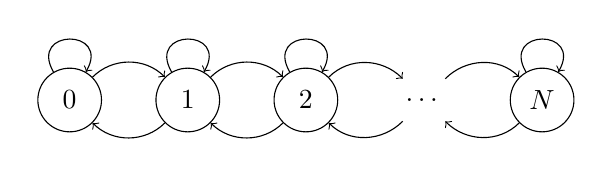
\begin{tikzpicture}[
			node distance={15mm},
			main/.style = {draw, circle, minimum size=23pt},
			dots/.style = {minimum size=15pt}
		]
		\node[main] (1) {$0$};
		\node[main] (2) [right of=1] {$1$};
		\node[main] (3) [right of=2] {$2$};
		\node[dots] (4) [right of=3] {$\dots$};
		\node[main] (5) [right of=4] {$N$};
		% For some reason using foreach doesn't align properly the edges on the \j node.
		%\foreach \i [evaluate=\i as \j using \i+1] in {1,2,3}  {
		%	\draw[->] (\i) to [out=120, in=60, looseness=4] (\i);
		%	\draw[->] (\i) to [out=45, in=135] (\j);
		%	\draw[->] (\j) to [out=225, in=315] (\i);
		%}
		\draw[->] (1) to [out=120, in=60, looseness=4] (1);
		\draw[->] (1) to [out=45, in=135] (2);
		\draw[->] (2) to [out=225, in=315] (1);
		\draw[->] (2) to [out=120, in=60, looseness=4] (2);
		\draw[->] (2) to [out=45, in=135] (3);
		\draw[->] (3) to [out=225, in=315] (2);
		\draw[->] (3) to [out=120, in=60, looseness=4] (3);
		\draw[->] (3) to [out=45, in=135] (4);
		\draw[->] (4) to [out=225, in=315] (3);
		\draw[->] (4) to [out=45, in=135] (5);
		\draw[->] (5) to [out=225, in=315] (4);
		\draw[->] (5) to [out=120, in=60, looseness=4] (5);
	\end{tikzpicture}
\end{center}
Θεωρούμε $\forall i \in S$ το $A = \{0,1,2,\dots,i\}$, τότε από τις εξισώσεις γενικευμένης ισορροπίας παίρνουμε
\begin{flalign}
	\sum_{j\in A} \sum_{i\in A^c} \pi_j p_{ji} = \sum_{i\in A^c} \sum_{j\in A} \pi_i p_{ij}
		&\Rightarrow \pi_{i-1} p_{i-1,i} = \pi_{i} p_{i,i-1}
		\Rightarrow \pi_{i-1} \frac{N-i+1}{N} p = \pi_i \frac{i}{N} q \notag &\\
		&\Rightarrow \pi_{i-1} (N-i+1) p = \pi_i i (1-p) \notag\\
		&\Rightarrow \pi_i = \pi_{i-1}\frac{N-i+1}{i} \cdot \frac{p}{1-p} \notag\\
		&\Rightarrow \pi_i = \frac{(N-i+1)(N-i+2) \cdots N}{i (i-1) \cdots 1} \left(\frac{p}{1-p}\right)^i \pi_0 \notag\\
		&\Rightarrow \pi_i = \binom{N}{i} \left(\frac{p}{1-p}\right)^i \pi_0 \label{eqpr2}
\end{flalign}
Από την εξίσωση κανονικοποίησης τώρα έχουμε
\begin{align*}
	\sum_{i=0}^N \pi_i = 1 &\Rightarrow \pi_0 + \sum_{i=1}^N \pi_i = 1
		\stackrel{\eqref{eqpr2}}{\Rightarrow} \pi_0 + \sum_{i=1}^N \binom{N}{i} \left(\frac{p}{1-p}\right)^i \pi_0 = 1 &\\
		&\Rightarrow \pi_0 \left(1 + \sum_{i=1}^N \binom{N}{i} \left(\frac{p}{1-p}\right)^i \right) = 1
		\Rightarrow \pi_0 \sum_{i=0}^N \binom{N}{i} \left(\frac{p}{1-p}\right)^i = 1\\
		&\Rightarrow \pi_0 \left(1+\frac{p}{1-p}\right)^N = 1
		\Rightarrow \pi_0 \left(\frac{1}{1-p}\right)^N = 1\\
		&\Rightarrow \pi_0 = (1-p)^N
\end{align*}
και άρα η στάσιμη κατανομή είναι το διάνυσμα $[\pi_i]_{i=0,1,\dots,N}$ όπου
\[
	\pi_i = \binom{N}{i} \left(\frac{p}{1-p}\right)^i (1-p)^N = \binom{N}{i} p^i (1-p)^{N-i}
\]

\paragraph{(δ)}
Το μακροπρόθεσμο ποσοστό του χρόνου που υπάρχουν $i$ σφαιρίδια στην κάλπη $A$ είναι
\[
	\lim_{n \rightarrow \infty} \frac{\sum_{k=0}^{n-1} 1_{\{X_k=i\}}}{n} = \pi_i = \binom{N}{i} p^i (1-p)^{N-i}
\]
\pagebreak

\section*{Άσκηση 3}

\paragraph{(α)}
\begin{center}
	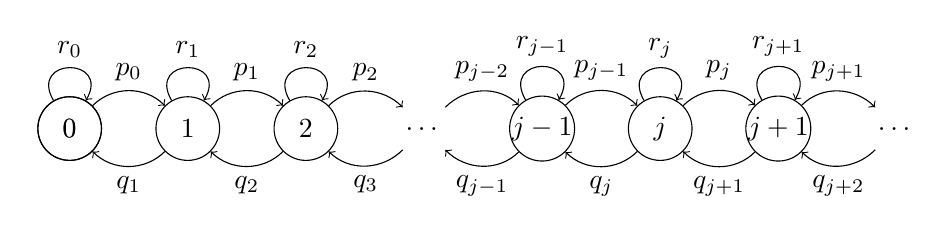
\begin{tikzpicture}[
			node distance={15mm},
			main/.style = {draw, circle, minimum size=23pt, inner sep=0pt},
			dots/.style = {minimum size=15pt}
		]
		\node[main] (1) {$0$};
		\node[main] (1) {$0$};
		\node[main] (2) [right of=1] {$1$};
		\node[main] (3) [right of=2] {$2$};
		\node[dots] (4) [right of=3] {$\dots$};
		\node[main] (5) [right of=4] {$j-1$};
		\node[main] (6) [right of=5] {$j$};
		\node[main] (7) [right of=6] {$j+1$};
		\node[dots] (8) [right of=7] {$\dots$};
		\draw[->] (1) to [out=120, in=60, looseness=4] node[above] {$r_0$} (1);
		\draw[->] (1) to [out=45, in=135] node[above] {$p_0$} (2);
		\draw[->] (2) to [out=225, in=315] node[below] {$q_1$} (1);
		\draw[->] (2) to [out=120, in=60, looseness=4] node[above] {$r_1$} (2);
		\draw[->] (2) to [out=45, in=135] node[above] {$p_1$} (3);
		\draw[->] (3) to [out=225, in=315] node[below] {$q_2$} (2);
		\draw[->] (3) to [out=120, in=60, looseness=4] node[above] {$r_2$} (3);
		\draw[->] (3) to [out=45, in=135] node[above] {$p_2$} (4);
		\draw[->] (4) to [out=225, in=315] node[below] {$q_3$} (3);
		\draw[->] (4) to [out=45, in=135] node[above] {$p_{j-2}$} (5);
		\draw[->] (5) to [out=225, in=315] node[below] {$q_{j-1}$} (4);
		\draw[->] (5) to [out=120, in=60, looseness=4] node[above] {$r_{j-1}$} (5);
		\draw[->] (5) to [out=45, in=135] node[above] {$p_{j-1}$} (6);
		\draw[->] (6) to [out=225, in=315] node[below] {$q_{j}$} (5);
		\draw[->] (6) to [out=120, in=60, looseness=4] node[above] {$r_j$} (6);
		\draw[->] (6) to [out=45, in=135] node[above] {$p_j$} (7);
		\draw[->] (7) to [out=225, in=315] node[below] {$q_{j+1}$} (6);
		\draw[->] (7) to [out=120, in=60, looseness=4] node[above] {$r_{j+1}$} (7);
		\draw[->] (7) to [out=45, in=135] node[above] {$p_{j+1}$} (8);
		\draw[->] (8) to [out=225, in=315] node[below] {$q_{j+2}$} (7);
	\end{tikzpicture}
\end{center}
Η Μ.Α.Δ.Χ. είναι αδιαχώριστη αφού $p_{i,i+1} > 0$ και $p_{i-1,i} > 0, i = 1,2,\dots$.
\\[8pt]
Τώρα αν για $j=1,2,\dots$ θεωρήσουμε το $A_j = \{0,1,2,\dots,j-1\}$, τότε από τις εξισώσεις γενικευμένης ισορροπίας παίρνουμε
\[
	\pi_{j-1} p_{j-1} = \pi_j q_j \Rightarrow \pi_j = \frac{p_{j-1}}{q_j} \pi_{j-1}
\]
και άρα
\begin{equation}
	\pi_j = \frac{p_{j-1} p_{j-2} \dots p_0}{q_j q_{j-1} \dots q_1} \pi_0 \label{eqpr3}
\end{equation}
Από την εξίσωση κανονικοποίησης τώρα παίρνουμε
\begin{align*}
	\sum_{j=0}^\infty \pi_j = 1 &\Rightarrow \pi_0 + \sum_{j=1}^\infty \pi_j = 1
		\stackrel{\eqref{eqpr3}}{\Rightarrow} \pi_0 + \sum_{j=1}^\infty \frac{p_{j-1} p_{j-2} \dots p_0}{q_j q_{j-1} \dots q_1} \pi_0 = 1 &\\
		&\Rightarrow \pi_0 \left(1 + \sum_{j=1}^\infty \frac{p_{j-1} p_{j-2} \dots p_0}{q_j q_{j-1} \dots q_1} \right) = 1
\end{align*}
Θέτουμε $B^{-1} = 1 + \sum_{j=1}^\infty \frac{p_{j-1} p_{j-2} \dots p_0}{q_j q_{j-1} \dots q_1}$ και έχουμε
\begin{itemize}
	\item αν $B^{-1} < \infty$ τότε υπάρχει στάσιμη κατανομή και άρα η Μ.Α.Δ.Χ. είναι θετικά επαναληπτική με
		\[\pi_0=B, \pi_j = \frac{p_{j-1} p_{j-2} \dots p_0}{q_j q_{j-1} \dots q_1} B, j \geq 1\]
	\item αν $B^{-1} = \infty$ τότε $\pi_j = 0, \forall j = 0,1,2,\dots$ οπότε δεν υπάρχει στάσιμη κατανομή και άρα η αλυσίδα δεν είναι θετικά επαναληπτική
\end{itemize}
Άρα η $\{X_n,n\geq 0\}$ είναι θετικά επαναληπτική αν και μόνον αν $B < \infty$.

\paragraph{(β)}
Από το (α) υποερώτημα έχουμε ήδη ότι αν $B^{-1} < \infty$ τότε η στάσιμη κατανομή είναι το διάνυσμα $[\pi_i]_{i=0,1,2,\dots}$ όπου
\[\pi_0=B, \pi_j = \frac{p_{j-1} p_{j-2} \dots p_0}{q_j q_{j-1} \dots q_1} B, j \geq 1\]


\section*{Άσκηση 4}

\paragraph{(α)}
\begin{center}
	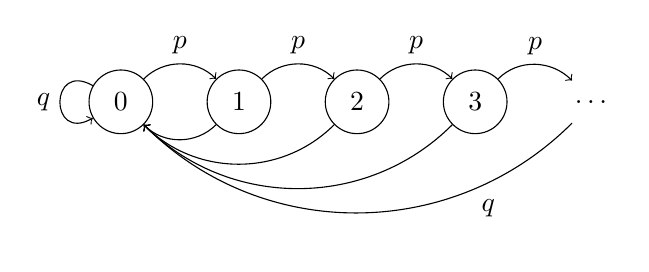
\begin{tikzpicture}[
			node distance={15mm},
			main/.style = {draw, circle, minimum size=23pt, inner sep=0pt},
			dots/.style = {minimum size=15pt}
		]
		\node[main] (1) {$0$};
		\node[main] (2) [right of=1] {$1$};
		\node[main] (3) [right of=2] {$2$};
		\node[main] (4) [right of=3] {$3$};
		\node[dots] (5) [right of=4] {$\dots$};
		\draw[->] (1) to [out=150, in=210, looseness=4] node[left] {$q$} (1);
		\draw[->] (1) to [out=45, in=135] node[above] {$p$} (2);
		\draw[->] (2) to [out=225, in=315] (1);
		\draw[->] (2) to [out=45, in=135] node[above] {$p$} (3);
		\draw[->] (3) to [out=225, in=315] (1);
		\draw[->] (3) to [out=45, in=135] node[above] {$p$} (4);
		\draw[->] (4) to [out=225, in=315] (1);
		\draw[->] (4) to [out=45, in=135] node[above] {$p$} (5);
		\draw[->] (5) to [out=225, in=315] node[near start, below right] {$q$} (1);
	\end{tikzpicture}
\end{center}
Αρχικά βλέπουμε ότι αν $p=1 \Rightarrow q=0$ τότε $p_{ij} = 0, \forall i > j$ και άρα η $\{X_n,n\geq 0\}$ δεν είναι επαναληπτική.
Άρα απαιτούμε $p<1 \Rightarrow q>0$, στη οποία περίπτωση η αλυσίδα είναι επαναληπτική αλλά και αδιαχώριστη.
\\[8pt]
Επίσης τότε η $\{X_n,n\geq 0\}$ και απεριοδική αφού $p_{00} = q > 0$.
\\[8pt]
Παίρνουμε τώρα τις εξισώσεις πλήρους ισορροπίας
\[
	\pi = \pi P \Rightarrow (\pi_0,\pi_1,\dots) = (\pi_0,\pi_1,\dots)
		\begin{pmatrix}
			q & p & 0 & 0 & \cdots\\
			q & 0 & p & 0 & \cdots\\
			q & 0 & 0 & p & \cdots\\
			\vdots & \vdots & \vdots & \vdots & \ddots
		\end{pmatrix}
		\Rightarrow
			\begin{dcases}
				\pi_0 = \sum_{j=0}^\infty \pi_j q\\
				\pi_1 = p \cdot \pi_0\\
				\pi_2 = p \cdot \pi_1 \\
				\vdots
			\end{dcases}
		\Rightarrow
			\begin{cases}
				\pi_0 = q\\
				\pi_1 = p \cdot q\\
				\pi_2 = p^2 \cdot q \\
				\vdots
			\end{cases}
\]
αφού από την εξίσωση κανονικοποίησης έχουμε $\sum_{j=0}^\infty \pi_j = 1$ και άρα
\[\pi_0 = \sum_{j=0}^\infty \pi_j q = q \sum_{j=0}^\infty \pi_j = q\]
Άρα υπάρχει στάσιμη κατανομή και η $\{X_n,n\geq 0\}$ είναι θετικά επαναληπτική αν και μόνον αν $p<1$.

\paragraph{(β)}
Από το (α) υποερώτημα έχουμε ήδη ότι αν $p<1$ τότε η στάσιμη κατανομή είναι το διάνυσμα $\pi = [\pi_i]_{i=0,1,2,\dots}$ όπου
\[\pi_i = p^i \cdot q\]

\pagebreak


\section*{Άσκηση 5}

Έστω $Y_n$ το υποσύνολο του $A$ που έχει επισκεφθεί η αλυσίδα μέχρι το $n$-οστό βήμα.\\
Η $\{(X_n,Y_n,n\geq 0)\}$ είναι Μ.Α.Δ.Χ. και θεωρούμε ότι απορροφάται όταν επισκεφθεί κατάσταση με $X_n=0$ ή $Y_n=A$.
Δηλαδή οι πιθανότητες μετάβασης της νέας Μ.Α.Δ.Χ. είναι
\begin{align*}
	&P(X_{n+1}=0,Y_{n+1}=B|X_n=0,Y_n=B) = 1\\
	&P(X_{n+1}=i,Y_{n+1}=A|X_n=i,Y_n=A) = 1\\
	&P(X_{n+1}=j,Y_{n+1}=C|X_n=i,Y_n=B) = p_{ij}
\end{align*}
με
\[C = \begin{cases}
	B \cup \{j\}, & j \in A-B\\
	B & j \notin A-B
\end{cases}\]
Για $B \subseteq A$ και $i \geq 1$ συμβολίζουμε με $p(i,B)$ την πιθανότητα η αλυσίδα να απορροφηθεί σε κατάσταση με $Y_n=A$ ξεκινώντας από την $(i,B)$.
Κάνοντας ανάλυση πρώτου βήματος παίρνουμε
\[
	\begin{dcases}
		p(i,B) = \sum_{j=0} p_{i_0} \cdot 0 + \sum_{j\in A-B} p_{ij} \cdot p(i,B\cup \{j\}) + \sum_{j\notin (A-B) \cup \{0\}} p_{ij} \cdot p(j,B)\\
		p(i,A) = 1
	\end{dcases}
\]
και αυτό $\forall i\in S \setminus \{0\}$ και $B \subseteq A$.
\\[8pt]
Η λύση του παραπάνω συστήματος μας δίνει τον υπολογισμό της $f_A$.
Πιο συγκεκριμένα, αν $\pi^{(0)}$ η αρχική κατανομή τότε λύνοντας το σύστημα παίρνουμε
\[
	f_A = \sum_{i\in A} \pi^{(0)}(i) \cdot p(i,\{i\}) + \sum_{i\notin A} \pi^{(0)}(i) \cdot p(i,\emptyset) + \pi^{(0)}(0) \cdot 0
\]

\end{document}
